\documentclass[a4paper,]{article}
\usepackage[left=2.5cm,top=2.5cm,right=2.5cm,bottom=3cm]{geometry} 
\usepackage[utf8]{inputenc}
\usepackage{graphicx} % Required for inserting images
\usepackage[table,xcdraw]{xcolor}
\usepackage{lipsum} % for dummy text
\usepackage{mathdots} % para el comando \iddots
\usepackage{mathrsfs} % para formato de letra
\usepackage{marvosym}
\usepackage{amsmath}
\DeclareUnicodeCharacter{2212}{-}


\title{\textbf{HW3: Introduction to Financial Engineering}}
\author{Miguel Angel Aguilo Gonzalez, 1699413 \\ Judit de Paz Ramírez, 1570590 \\ Laia Mòdol Rodríguez, 1565282 \\ Elena Rubio Zabala, 1699049 \\ Guillem Tutusaus Alcaraz, 1533701 } 
\date{Noviembre 2023}

\begin{document}

\maketitle
\newpage

\section*{Exercise 1}
\textbf{Complete the following questionnaire for each of the option strategies (there are 7 different strategies) (all strategies have the same expiry and are written on the same underlying, consider the spot price to be 100):}

\begin{enumerate}
    \item \textbf{Write down the payoff function in formulas (without premiums).}
    \item \textbf{Plot the payoff function without premiums (show in different colours the building blocks of the stategy and the aggegated result).}
    \item \textbf{Investigate and explain in your own words the financial rationale of the strategy.}
    \item \textbf{Plot a profit diagram for arbitrary premiums (although arbitrary, premium must fulfil the right order and magnitude between them).}
\end{enumerate}

\begin{itemize}
    \item[\textbf{(a)}] \textbf{Bull Spread:} We buy a Call at 100 and sell one at 120. The formula looks like this:
    \[ 
    P(t)=
    \begin{cases} 
      \frac{20}{100}x & S(t)\geq 120 \\
      \frac{S(t)-100}{100}x & 120\geq S(t)\geq 100 \\
      0 & 100\geq S(t) 
   \end{cases}
    \]
    $P(t)=\text{Payoff function}$\\
    $S(t)=\text{stock price at instant t}$\\
    $x=\text{number of stocks for the price, that is} 100n$


   For the plots we consider $n=1$.
    
    \vspace{3mm}
    \noindent
    
    The Bull Spread is a strategy that allows us to limit losses, but also profits. That is why it is very useful when we work with price ranges where we think the quote will go up. We use the Bull Spread if we think the stock's rise is moderate. If we believe or sense that the increase will be very large, there is no point in taking a Bull Spread, as we would benefit more from buying the Call cheap and letting it grow. It is true that if we sold the Call high we would limit the possibility of winning more, but we would also cut the initial premium by reaching the breakout point earlier. This is why the Bull Spread is considered an optimistic strategy.
    
    \vspace{3mm}
    \noindent
    In the plot with premium you can see how the breakout point must be reached to compensate for the cost of the operation.
    
    \begin{center}
        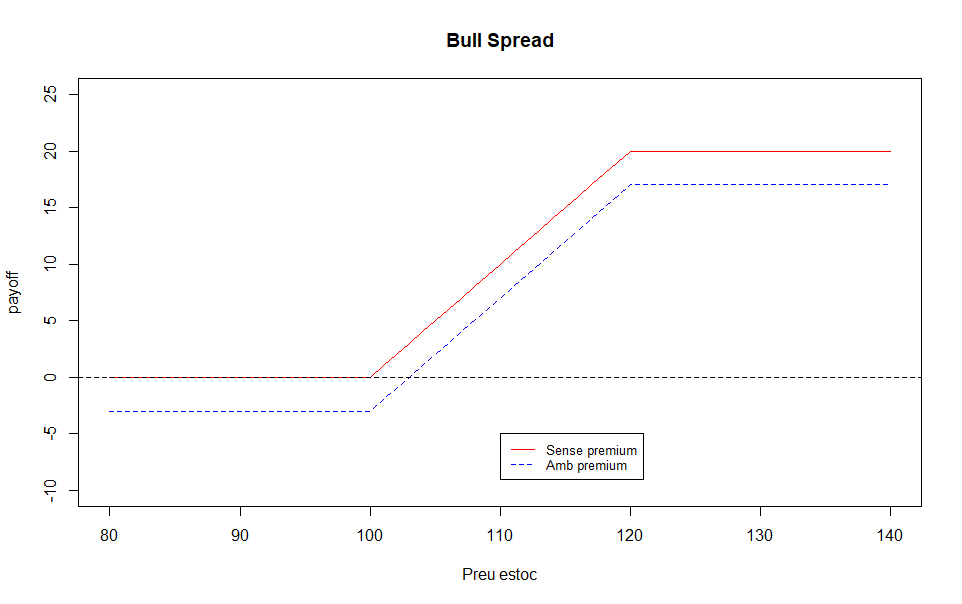
\includegraphics[scale=0.5]{Bull Spread.png}
    \end{center}
    
    \item[\textbf{(b)}] \textbf{Bear Spread:} We sell a Put at 100 and buy one at 120. The formula remains like this, with the same parameters as before.
    
    \[ 
    P(t)=
    \begin{cases}
        \frac{20}{100}x & 100\geq S(t) \\
        \frac{S(t)-100}{100}x & 120\geq S(t)\geq 100 \\
        0 & 120\geq S(t) 
    \end{cases}
    \]

    \vspace{3mm}
    \noindent
    The Bear Spread, like the Bull strategy, consists of two Puts (one bought, the other sold and both with the same expiration date). The difference is that the Bear Spread takes advantage of a moderate decline in the stock price and we follow the same strategy as the Bull Spread, but in reverse: here we compensate for premium prices while limiting profits. This strategy is considered a neutral-low strategy.
    
    \vspace{3mm}
    \noindent
    In the following plot it is seen in red without premiums and in blue with, in the latter we can see how the breakout point must be reached to compensate for the cost of the operation.

    \begin{center}
        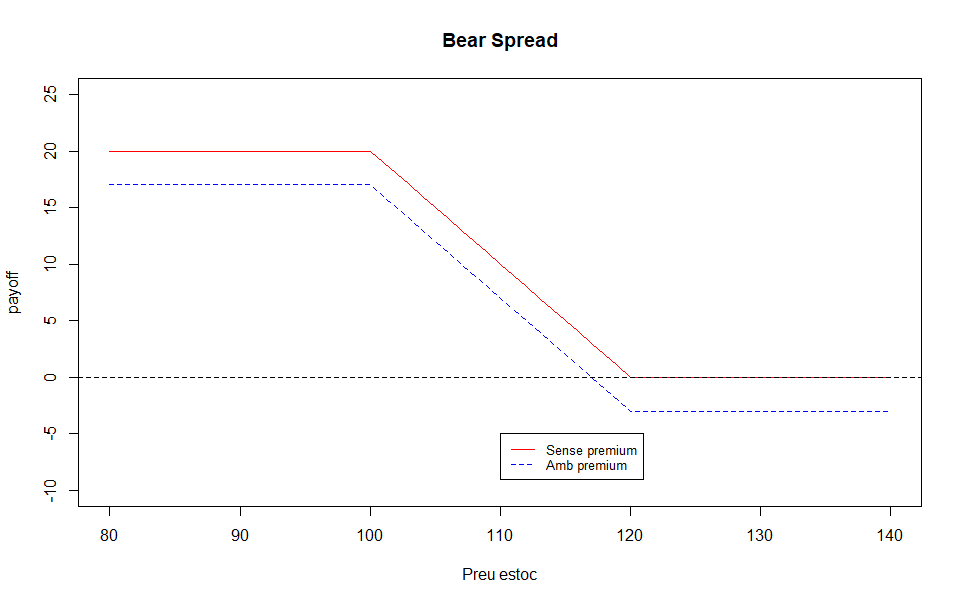
\includegraphics[scale=0.5]{Bear Spread.png}
    \end{center}

    \item[\textbf{(c)}] \textbf{Covered Call:} We have a unit of the stock and we sell a Call at 110, that's the formula

    \[ 
    P(t)=
    \begin{cases}
        \frac{10}{100}x & S(t)\geq 110 \\
        \frac{S(t)-100}{100}x & 110\geq S(t)
    \end{cases}
    \]

    A Covered Call is a strategy used to generate income in the form of option premiums. Investors expect an increase in the price of the underlying stock during the life of the option. The goal is to make money with the premium without being forced to sell it at the strike price, although the funny thing is that if the case were to happen, we are covered (hence the name Covered Call), since we have the stock . If we don't cover ourselves by buying a call option we would have a potential loss in the value of the stock so at the moment it is one of the riskiest strategies we have seen. The premium is positive. So we would have:

    \begin{center}
        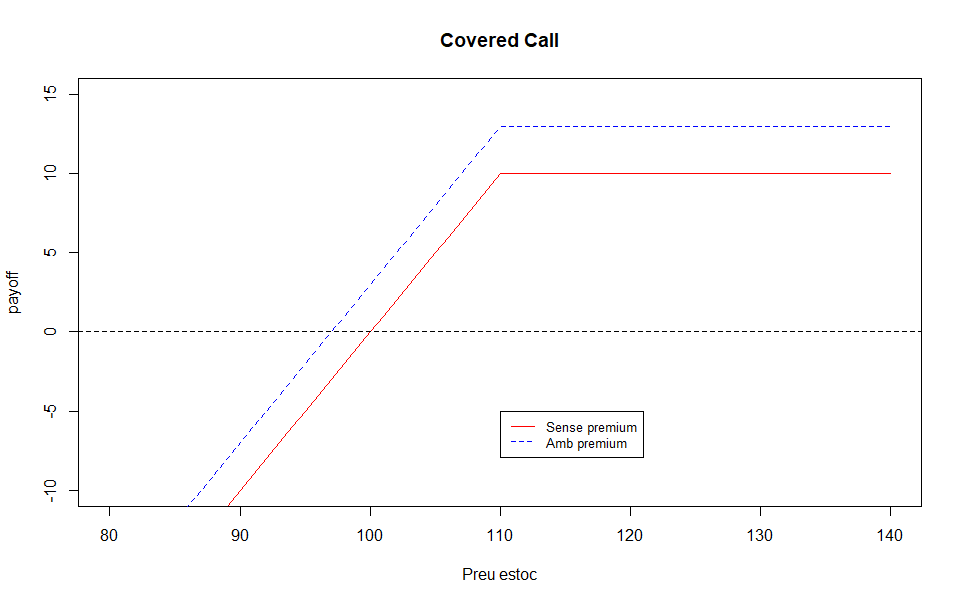
\includegraphics[scale=0.5]{Covered Call.png}
    \end{center}

    \item[\textbf{(d)}] \textbf{Covered Put:} We short sell one unit of the stock and sell a Put at 90, the formula would be:

    \[ 
    P(t)=
    \begin{cases}
        \frac{10}{100}x & 90\geq S(t) \\
        \frac{S(t)-100}{100}x & S(t)\geq 90
    \end{cases}
    \]

   In the reverse of the Covered Call, when we think a stock will decrease, but only a little, in this case, not below 90, we take advantage of the premium of selling the Put to make money. This is a risky strategy because theoretically here the losses are not fixed. So the plots remain:

    \begin{center}
        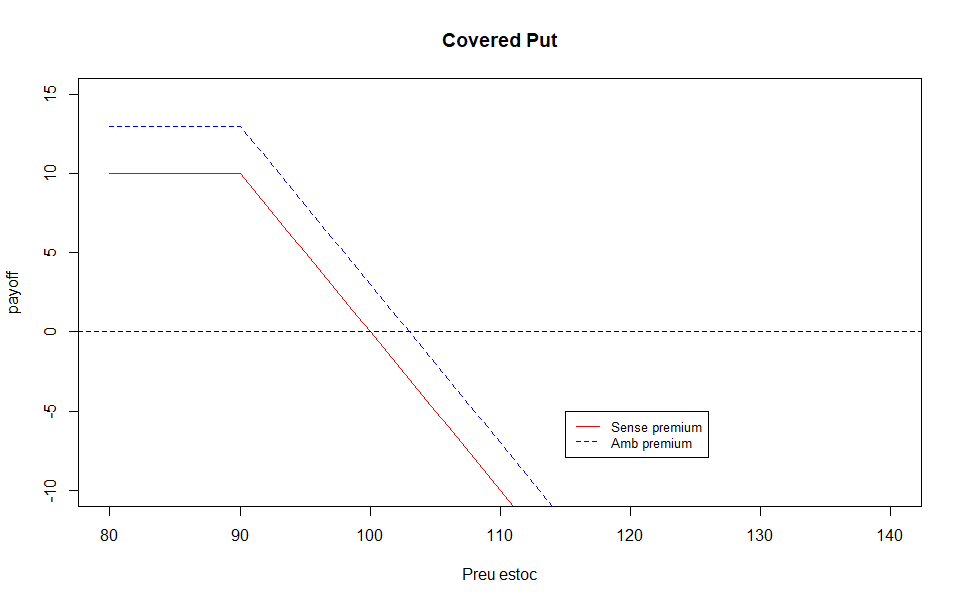
\includegraphics[scale=0.5]{Covered Put.png}
    \end{center}

    \item[\textbf{(e)}] \textbf{Collar:} If we have one unit of the stock, sell a Call at 110 and buy a Put at 90, the formula looks like this.

    \[ 
    P(t)=
    \begin{cases}
        \frac{10}{100}x & S(t)\geq 110 \\
        \frac{S(t)-100}{100}x & 110\geq S(t)\geq 90 \\
        \frac{-10}{100}x & 90\geq S(t)
    \end{cases}
    \]

    \vspace{3mm}
    \noindent
   The Collar is a strategy we use to protect ourselves. We use it when we think there will be fluctuations in the market. That is why the collar strategy is used when we are in long processes because we are interested in keeping the units of the stock. Sometimes we can even get a 0 premium just to cover our backs.

    \vspace{3mm}
    \noindent
   The plots with and without premium are:

    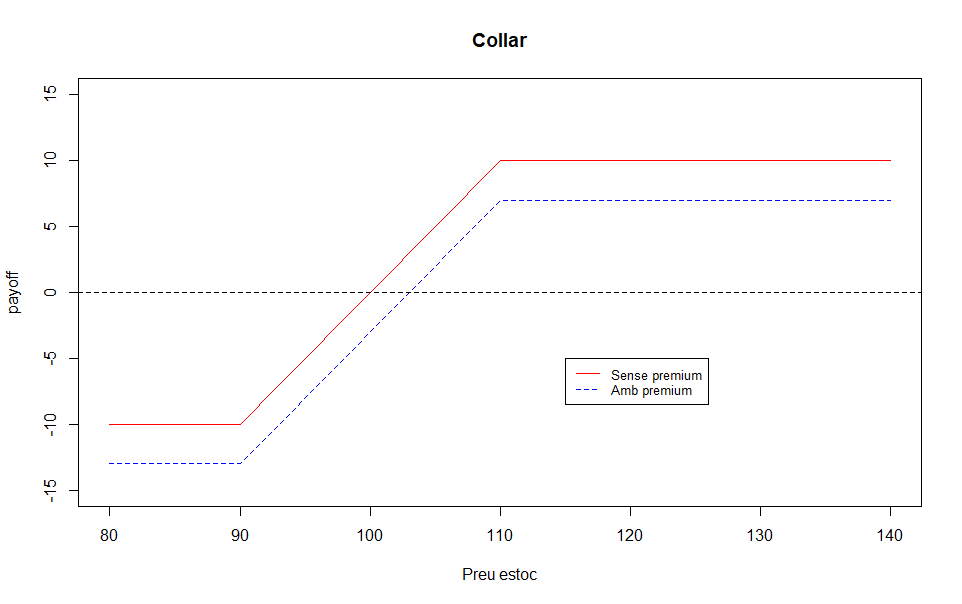
\includegraphics[scale=0.5]{Collar.png}

    \item[\textbf{(f)}] \textbf{Butterfly:} We sell a Put at 90, buy a Call at 100 and a Put at 100, and sell a Call at 110.

    \[ 
    P(t)=
    \begin{cases}
        0 & 90\geq S(t) \\
        \frac{S(t)-90}{100}x & 100\geq S(t)\geq 90 \\
        \frac{110-S(t)}{100}x & 110\geq S(t)\geq 100 \\
        0 & S(t)\geq 110
    \end{cases}
    \]

    This strategy serves us to profit from a stock that we believe will not move much from the range it is in and is a strategy with limited risk and profit.

    \vspace{3mm}
    \noindent
    Els plots són els següents:

    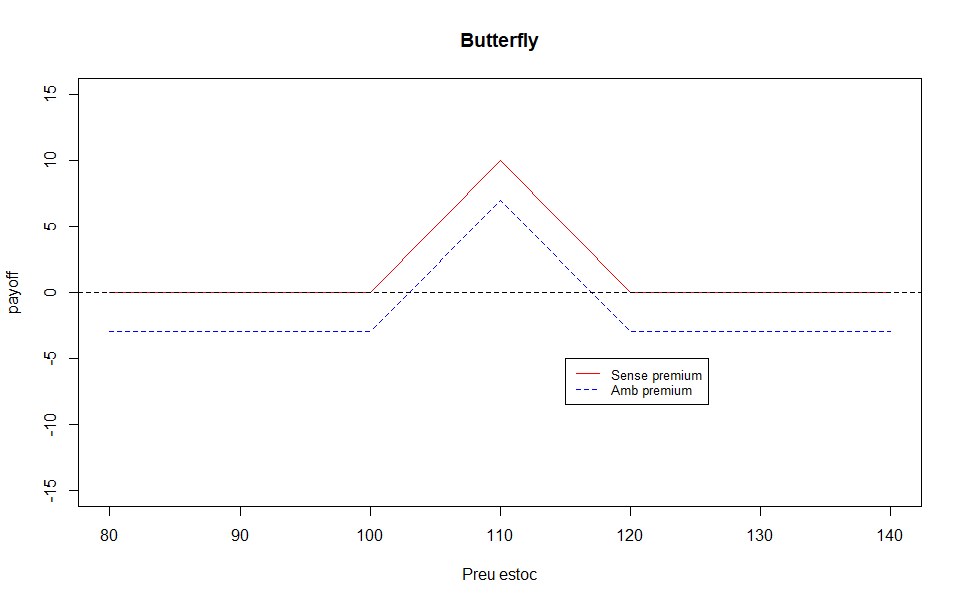
\includegraphics[scale=0.5]{Butterfly.png}

    \item[\textbf{(g)}] \textbf{Condor:} We sell a Call at 90, buy a Call at 100 and a Put at 100 and sell a Call at 110, then the function remains:

    \[ 
    P(t)=
    \begin{cases}
        0 & 90\geq S(t) \\
        \frac{S(t)-90}{100}x & 100\geq S(t)\geq 90 \\
        \frac{20}{100}x & 110\geq S(t)\geq 100 \\
        \frac{110-S(t)}{100}x & 120\geq S(t)\geq 110 \\
        0 & S(t)\geq 120
    \end{cases}
    \]

    The Condor is a useful strategy for when we think the stock is not going to move much as in the case of the Butterfly. This one, however, gives us a wider range of movement.

    \vspace{3mm}
    \noindent
    The plot looks like this:

    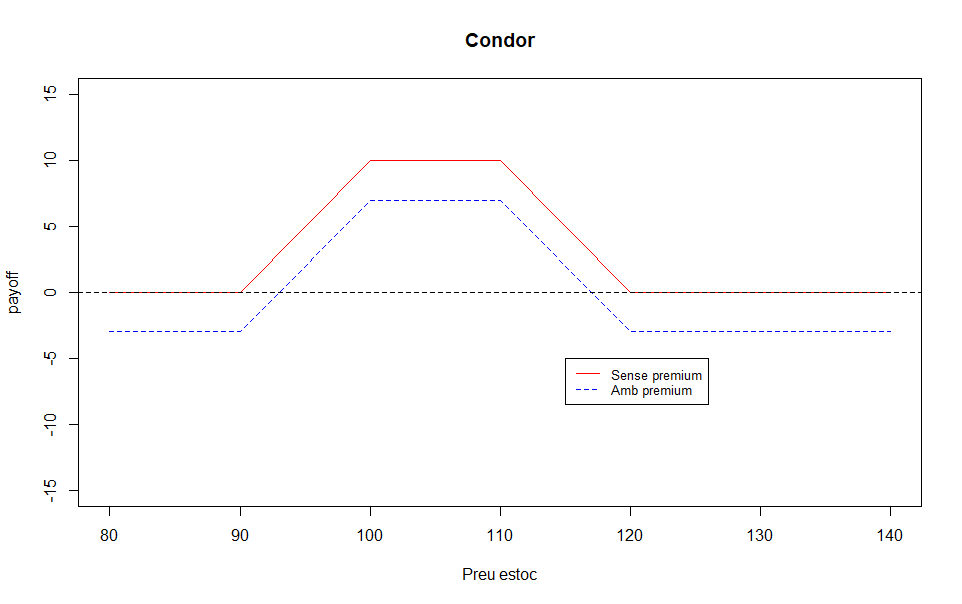
\includegraphics[scale=0.5]{Condor.png}
\end{itemize}

\newpage
\section*{Exercise 2}

\textbf{A stock currently trades at $60\$$. A Call with strike price $58\$$ and expiry 12 months trades at $3\$$; a Put with the same strike and expiry trades at $2\$$. The interest rate at 12 months is $10\$$.}

\vspace{3mm}
\noindent
The put-call parity is an important concept for every person who is dedicated to operating with shares. This parity characterizes the share price. Hans Stoll who was the first to document this, in a report called "The Relation Between Put and Call Prices" in 1969, said that the premium of a call stock implied a certain fair price for the corresponding put option with the same strike and expiration date and the same for the reverse. In other words; The put-call parity is a relationship between call options, put options and their underlying price. So it guarantees that at all times there must be a balance between them and when this parity is out of tune, that's when arbitrage opportunities appear. The formula that determines this relationship is as follows:

$$c_0+\frac{X}{e^{rT}}=p_0+S_0$$

\noindent
$c_0=\text{price of call today}$\\
$p_0=\text{price of put today}$\\
$X=\text{Strike price}$\\
$S_0=\text{price of underlying stock today}$\\
$r=\text{risk-free rate}$\\
$T=\text{Time in years}$

\begin{itemize}
    \item \textbf{Do any arbitrage opportunities exist?}

    Let's calculate the equation in our experiment:

    $$c_0+\frac{X}{e^{rT}}=3+\frac{58}{e^{0.1}}=55.48$$
    $$p_0+S_0=58+2=60$$

    Given that the two members of equality are not equal, we affirm that there is some arbitrage opportunity.

    \item \textbf{If there is a possible arbitrage, then explain the strategy to get profit from it.}

   In these cases, the way to profit from arbitration is always the same. Sell the more expensive wallet and buy the cheaper one.
    \vspace{3mm}
    \noindent
    In our experiment, we would sell the protective put $60\$$ and  buy the fiduciary call $55.48\$$, generating a cash inflow of: $60-55.48 = 4.52\$$ and no cash outflow. Studying the Payoff maturity we can see that there is no cash outflow:

    \begin{table}[ht]
    \centering
    \begin{tabular}{|c|c|c|}
    \textbf{Payoff from} & $S_T\leq 58$ & $S_T> 58$ \\
    \textbf{Call} & $0\$$ & $S_T-58\$$ \\
    \textbf{Risk-free bond} & $58\$$ & $58\$$ \\
    \textbf{Total} & $58\$$ & $S_T$ \\
    \end{tabular}
    \caption{Payoff from fiduciary call: $c_0+\frac{X}{e^{rT}}$}
    \end{table}

    \begin{table}[ht]
    \centering
    \begin{tabular}{|c|c|c|}
    \textbf{Payoff from} & $S_T\leq 58$ & $S_T> 58$ \\
    \textbf{Stock} & $S_T$ & $S_T$ \\
    \textbf{Put} & $58\$-S_T$ & $0$ \\
    \textbf{Total} & $58\$$ & $S_T$ \\
    \end{tabular}
    \caption{Payoff from protective put: $p_0+S_0$}
    \end{table}
\end{itemize}

%Supongamos que una acción cotiza actualmente a 60\$. Supongamos tambiés que un "Call" con "strike" 58\$ y tiene fecha límite en 12 meses que cotiza a 3\$. También tenemos un "Put" con el mismo "Strike" y vencimiento que cotiza a 2\$. La tasa de interés a 12 meses es del 10\%. Queremos ver si hay arbitraje, es decir, si se puede sacar provecho de una diferencia de precio entre dos o más mercados, observando  la paridad put-call. Teniendo C como precio de "Call", P como precio de "Put", S como precio al contado hoy y F como precio a plazo. Veamos si hay paridad:
%$$C(t)-P(t)=S(t)-F(t)=S(t)-Ke^{-r(T-t)}  \Leftrightarrow 3-2=60-58e^{-0.1} \Leftrightarrow 1=7.519     !!! $$
%Ya que la igualdad no se cumple, deduciomos existe una oportunidad de arbitraje.\\

%La idea básica para hacer dinero es la de comprar barato y vender caro, por tanto haremos exactamente esto, compraremos la Call (sería comprar barato) y venderemos la Put option (vender caro). Si reordenamos un poco las fórmulas y siguiendo los conceptos mencionados en la práctica para las Put y Call options nos quedaría la siguiente tabla:

%\begin{center}
%\begin{tabular}{|l|l|l|}
%\hline
%\textbf{Posició}     & \textbf{Valor a l'instant $t_o$} & \textbf{Valor a l'instant $T$} \\ \hline
%\textbf{Call Option} & $3$                              & max$(S(t)-58,0)$               \\ \hline
%\textbf{-Put Option} & $-2$                             & $-$max$(S(t)-58,0)$              \\ \hline
%\textbf{-Stock}      & $-60$                            & $S(T)$                         \\ \hline
%\textbf{Efectiu}     & $58e^{-0.1}=52.48$               & $58$                           \\ \hline
%\textbf{Total}                & $-6.52$                          & $0$                            \\ \hline
%\end{tabular}
%\end{center}

\end{document}



